\begin{frame}[fragile]
\frametitle{Aliasing loads (TMU)}
\begin{minipage}{0.7\textwidth}
\begin{minted}[escapeinside=||,mathescape=true,linenos]{c}
// Scope $\scope{h}$
void h(int* q, int* restrict r, int* restrict s) {
    *q = *r + *s; 
}
// Scope $\scope{main}$
int main() {
    int x, y;
    int* restrict p = &y;
    *p = 0; 
    h(&x, p, p);
}
\end{minted}
\end{minipage}%
\begin{minipage}[t]{0.3\textwidth}
\begin{tikzpicture}
    \node (q) {\mintinline{c}{q}};
    \node[right of = q] (pointee-q) {$x$};

    \node[right of = pointee-p] (rs) {\mintinline{c}{r,s}};
    \node[right of = rs] (pointee-rs) {$y$};

    \draw[->] (q) -- (pointee-q);
    \draw[->] (rs) -- (pointee-rs);
\end{tikzpicture}
\end{minipage}

\begin{itemize}
    \item Simplified version of example 3 from the ISO standard demonstrating DB
    \item $y$ does \textbf{not} get \textbf{modified} in the scope \scope{h} of \mintinline{c}{r,s}
\end{itemize}

\end{frame}


% ----


\begin{frame}[fragile]
\frametitle{Aliasing loads (TMU)}
\begin{minted}[escapeinside=||,mathescape=true]{c}
// Scope $\scope{h}$
void h(int* q, int* restrict r, int* restrict s) {
    *q = *r + *s; 
}
\end{minted}

\begin{figure}[h]
\centering
\begin{minipage}{.36\textwidth}
\begin{minted}[escapeinside=||,mathescape=true]{c}
// Scope $\scope{main}$
|\colorbox{red!20}{int main() \{}|
    int x, y;
    int* restrict p = &y;
    *p = 0; 
    h(&x, p, p);
}
\end{minted}
\end{minipage}%
\begin{minipage}{.674\textwidth}
\executionannotation
{
    $\emptyset$
}
{
    \begin{tikzpicture}[stack/.style={rectangle split, rectangle split parts=#1, draw, anchor=center, text centered},
        scope/.style={fill=gray!20, anchor=center}]
    \node[stack=1, minimum width=4.0cm] (s) {
    \nodepart{one} $\emptyset$
    };
    \node[scope, left=5pt of s.one west]   {\colorbox{red!20}{\scope{main}}};
    \end{tikzpicture}   
}
\end{minipage}
\end{figure}

\end{frame}


% ----


\begin{frame}[fragile]
\frametitle{Aliasing loads (TMU)}
\begin{minted}[escapeinside=||,mathescape=true]{c}
// Scope $\scope{h}$
void h(int* q, int* restrict r, int* restrict s) {
    *q = *r + *s; 
}
\end{minted}

\begin{figure}[h]
\centering
\begin{minipage}{.36\textwidth}
\begin{minted}[escapeinside=||,mathescape=true]{c}
// Scope $\scope{main}$
int main() {
    |\colorbox{red!20}{int x, y;}|
    int* restrict p = &y;
    *p = 0; 
    h(&x, p, p);
}
\end{minted}
\end{minipage}%
\begin{minipage}{.64\textwidth}
\executionannotation
{
\{\colorbox{red!20}{$\Blockvar_x \mapsto \vundef, \Blockvar_y \mapsto \vundef$}\}
}
{
    \begin{tikzpicture}[stack/.style={rectangle split, rectangle split parts=#1, draw, anchor=center, text centered},
        scope/.style={fill=gray!20, anchor=center}]
    \node[stack=1, minimum width=4.0cm] (s) {
    \nodepart{one} $\emptyset$
    };
    \node[scope, left=5pt of s.one west]   {\scope{main}};
    \end{tikzpicture}   
}
\end{minipage}
\end{figure}

\end{frame}


% ---- 


\begin{frame}[fragile]
\frametitle{Aliasing loads (TMU)}
\begin{minted}[escapeinside=||,mathescape=true]{c}
// Scope $\scope{h}$
void h(int* q, int* restrict r, int* restrict s) {
    *q = *r + *s; 
}
\end{minted}

\begin{figure}[h]
\centering
\begin{minipage}{.36\textwidth}
\begin{minted}[escapeinside=||,mathescape=true]{c}
// Scope $\scope{main}$
int main() {
    int x, y;
    |\colorbox{red!20}{int* restrict p = &y;}|
    *p = 0;
    h(&x, p, p);
}
\end{minted}
\end{minipage}%
\begin{minipage}{.64\textwidth}
\executionannotation
{
\{$\Blockvar_x \mapsto \vundef$, \\
    \ $\Blockvar_y \mapsto \vundef$, \\
    \ \colorbox{red!20}{$\Blockvar_p \mapsto \ptr{(\Blockvar_y, \set{(\Blockvar_p, \scope{main})})}$}
\}
}
{
    \begin{tikzpicture}[stack/.style={rectangle split, rectangle split parts=#1, draw, anchor=center, text centered},
        scope/.style={fill=gray!20, anchor=center}]
    \node[stack=1, minimum width=4.0cm] (s) {
    \nodepart{one} $\emptyset$
    };
    \node[scope, left=5pt of s.one west]   {\scope{main}};
    \end{tikzpicture}   
}
\end{minipage}
\end{figure}


\end{frame}


% ---- 


\begin{frame}[fragile]
\frametitle{Aliasing loads (TMU)}
\begin{minted}[escapeinside=||,mathescape=true]{c}
// Scope $\scope{h}$
void h(int* q, int* restrict r, int* restrict s) {
    *q = *r + *s; 
}
\end{minted}

\begin{figure}[h]
\centering
\begin{minipage}{.36\textwidth}
\begin{minted}[escapeinside=||,mathescape=true]{c}
// Scope $\scope{main}$
int main() {
    int x, y;
    int* restrict p = &y;
    |\colorbox{red!20}{*p = 0;}|
    h(&x, p, p);
}
\end{minted}
\end{minipage}%
\begin{minipage}{.64\textwidth}
\executionannotation
{
\{$\Blockvar_x \mapsto \vundef$, \\
    \ $\Blockvar_y \mapsto \colorbox{red!20}{0}$, \\
    \ $\Blockvar_p \mapsto \ptr{(\Blockvar_y, \set{(\Blockvar_p, \scope{main})})}$
\}
}
{
    \begin{tikzpicture}[stack/.style={rectangle split, rectangle split parts=#1, draw, anchor=center, text centered},
        scope/.style={fill=gray!20, anchor=center}]
    \node[stack=1, minimum width=4.0cm] (s) {
    \nodepart{one} \{\colorbox{red!20}{$\Blockvar_y \mapsto \restricted{\set{(\Blockvar_p, \scope{main})}}$}\}
    };
    \node[scope, left=5pt of s.one west]   {\scope{main}};
    \end{tikzpicture}   
}
\end{minipage}
\end{figure}


\end{frame}


% ---- 


\begin{frame}[fragile]
\frametitle{Aliasing loads (TMU)}
\begin{minted}[escapeinside=||,mathescape=true]{c}
// Scope $\scope{h}$
void h(int* q, int* restrict r, int* restrict s) {
    *q = *r + *s; 
}
\end{minted}
\vspace*{-1cm}
\begin{figure}[h]
\centering
\begin{minipage}{.36\textwidth}
\begin{minted}[escapeinside=||,mathescape=true]{c}
// Scope $\scope{main}$
int main() {
    int x, y;
    int* restrict p = &y;
    *p = 0;
    |\colorbox{red!20}{h(&x, p, p);}|
}
\end{minted}
\end{minipage}%
\begin{minipage}{.64\textwidth}
\executionannotation
{
\{$\Blockvar_x \mapsto \vundef$, $\Blockvar_y \mapsto 0$, \\
    \ $\Blockvar_p \mapsto \ptr{(\Blockvar_y, \set{(\Blockvar_p, \scope{main})})}$, \\
    \ \colorbox{red!20}{$\Blockvar_q \mapsto \ptr{(\Blockvar_x, \emptyset)}$}, \\
    \ \colorbox{red!20}{$\Blockvar_r \mapsto \ptr{(\Blockvar_y, \set{(\Blockvar_r, \scope{h}), (\Blockvar_p, \scope{main})})} $}, \\
    \ \colorbox{red!20}{$\Blockvar_s \mapsto \ptr{(\Blockvar_y, \set{(\Blockvar_s, \scope{h}), (\Blockvar_p, \scope{main})})} $} \\
\}
}
{
    \begin{tikzpicture}[stack/.style={rectangle split, rectangle split parts=#1, draw, anchor=center, text centered},
        scope/.style={fill=gray!20, anchor=center}]
    \node[stack=2, minimum width=4.0cm] (s) {
    \nodepart{one} $\emptyset$
    \nodepart{two} \{$\Blockvar_y \mapsto \restricted{\set{(\Blockvar_p, \scope{main})}}$\}
    };
    \node[scope, left=5pt of s.one west]   {\colorbox{red!20}{\scope{h}}};
    \node[scope, left=5pt of s.two west]   {\scope{main}};
    \end{tikzpicture}   
}
\end{minipage}
\end{figure}

\end{frame}



% ---- 


\begin{frame}[fragile]
\frametitle{Aliasing loads (TMU)}
\begin{minted}[escapeinside=||,mathescape=true]{c}
// Scope $\scope{h}$
void h(int* q, int* restrict r, int* restrict s) {
    *q = |\colorbox{red!20}{*r}| + *s; 
}
\end{minted}
\vspace*{-1cm}
\begin{figure}[!h]
\begin{minipage}[t]{.36\textwidth}

\begin{minted}[escapeinside=||,mathescape=true]{c}
// Scope $\scope{main}$
int main() {
    int x, y;
    int* restrict p = &y;
    *p = 0;
    h(&x, p, p);
}
\end{minted}
\end{minipage}%
\begin{minipage}{.64\textwidth}
\executionannotation
{
\{$\Blockvar_x \mapsto \vundef$, $\Blockvar_y \mapsto 0$, \\
    \ $\Blockvar_p \mapsto \ptr{(\Blockvar_y, \set{(\Blockvar_p, \scope{main})})}$, \\
    \ $\Blockvar_q \mapsto \ptr{(\Blockvar_x, \emptyset)}$, \\
    \ $\Blockvar_r \mapsto \ptr{(\Blockvar_y, \set{(\Blockvar_r, \scope{h}), (\Blockvar_p, \scope{main})})} $, \\
    \ $\Blockvar_s \mapsto \ptr{(\Blockvar_y, \set{(\Blockvar_s, \scope{h}), (\Blockvar_p, \scope{main})})} $ \\
\}
}
{
    \begin{tikzpicture}[stack/.style={rectangle split, rectangle split parts=#1, draw, anchor=center, text centered},
        scope/.style={fill=gray!20, anchor=center}]
    \node[stack=2, minimum width=4.0cm] (s) {
    \nodepart{one} \{\colorbox{red!20}{$\Blockvar_y \mapsto \onlyread{\set{(\Blockvar_r, \scope{h}), (\Blockvar_p, \scope{main})}}$}\}
    \nodepart{two} \{$\Blockvar_y \mapsto \restricted{\set{(\Blockvar_p, \scope{main})}}$\}
    };
    \node[scope, left=5pt of s.one west]   {\scope{h}};
    \node[scope, left=5pt of s.two west]   {\scope{main}};
    \end{tikzpicture}   
}
\end{minipage}
\end{figure}

\end{frame}

% ---- 


\begin{frame}[fragile]
\frametitle{Aliasing loads (TMU)}
\begin{minted}[escapeinside=||,mathescape=true]{c}
// Scope $\scope{h}$
void h(int* q, int* restrict r, int* restrict s) {
    *q = *r + |\colorbox{red!20}{*s}|; 
}
\end{minted}
\vspace*{-1cm}
\begin{figure}[!h]
\begin{minipage}[t]{.36\textwidth}

\begin{minted}[escapeinside=||,mathescape=true]{c}
// Scope $\scope{main}$
int main() {
    int x, y;
    int* restrict p = &y;
    *p = 0;
    h(&x, p, p);
}
\end{minted}
\end{minipage}%
\begin{minipage}{.64\textwidth}
\colorbox{red!20}{$\onlyread{\set{(\Blockvar_\text{\textcolor{blue}{$r$}}, \scope{h}), (\Blockvar_p, \scope{main})}} \joinsym $} \\
\colorbox{red!20}{$\onlyread{\set{(\Blockvar_\text{\textcolor{blue}{$s$}}, \scope{h}), (\Blockvar_p, \scope{main})}} = ...$}
\\

\executionannotation
{
\{..., \\\  $\Blockvar_r \mapsto \ptr{(\Blockvar_y, \set{(\Blockvar_r, \scope{h}), (\Blockvar_p, \scope{main})})} $, \\
         \ $\Blockvar_s \mapsto \ptr{(\Blockvar_y, \set{(\Blockvar_s, \scope{h}), (\Blockvar_p, \scope{main})})}$ \}
}
{
    \begin{tikzpicture}[stack/.style={rectangle split, rectangle split parts=#1, draw, anchor=center, text centered},
        scope/.style={fill=gray!20, anchor=center}]
    \node[stack=2, minimum width=4.0cm] (s) {
    \nodepart{one} \{$\Blockvar_y \mapsto \onlyread{\set{(\Blockvar_r, \scope{h}), (\Blockvar_p, \scope{main})}}$\}
    \nodepart{two} \{$\Blockvar_y \mapsto \restricted{\set{(\Blockvar_p, \scope{main})}}$\}
    };
    \node[scope, left=5pt of s.one west]   {\scope{h}};
    \node[scope, left=5pt of s.two west]   {\scope{main}};
    \end{tikzpicture}   
}
\end{minipage}
\end{figure}

\end{frame}


% ----


\begin{frame}[fragile]
\frametitle{Aliasing loads (TMU)}
\centering
\colorbox{red!20}{$\onlyread{\set{(\Blockvar_\text{\textcolor{blue}{$r$}}, \scope{h}), (\Blockvar_p, \scope{main})}} \joinsym \ \onlyread{\set{(\Blockvar_\text{\textcolor{blue}{$s$}}, \scope{h}), (\Blockvar_p, \scope{main})}} = \unrestricted$}

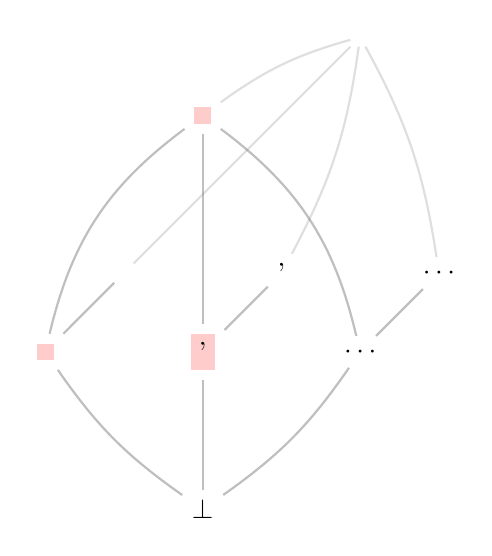
\begin{tikzpicture}
    \node (ub)     at (7,5) {\rsub};
    \node (un)     at (5,4) {\colorbox{red!20}{\unresabbr}};
    \node (rsbs)   at (4,2) {\resabbr{\Basesvar}};
    \node (rsbs')  at (6,2) {\resabbr{\Basesvar'}};
    \node (rsbs'') at (8,2) {$\cdots$};
    \node (orbs)   at (3,1) {\colorbox{red!20}{\orabbr{\Basesvar}}};
    \node (orbs')  at (5,1) {\colorbox{red!20}{\orabbr{\Basesvar'}}};
    \node (orbs'') at (7,1) {$\cdots$};
    \node (bot)    at (5,-1) {$\bot$};

    \path[thick, black, opacity=0.25]
    (bot) edge[bend left=10] node {} (orbs)
    (bot) edge node {} (orbs')
    (bot) edge[bend right=10] node {} (orbs'')
    
    (orbs) edge node {} (rsbs) 
    (orbs') edge node {} (rsbs')
    (orbs'') edge node {} (rsbs'')  
    
    (orbs) edge[bend left=20] node {} (un)
    (orbs') edge node {} (un)
    (orbs'') edge[bend right=20] node {} (un)

    (rsbs) edge[gray] node {} (ub)
    (rsbs') edge[bend right=10, gray] node {} (ub)
    (rsbs'') edge[bend right=10, gray] node {} (ub)

    (un) edge[bend left=10, gray] node {} (ub);
\end{tikzpicture}

\end{frame}

    
% ---- 


\begin{frame}[fragile]
\frametitle{Aliasing loads (TMU)}
\begin{minted}[escapeinside=||,mathescape=true]{c}
// Scope $\scope{h}$
void h(int* q, int* restrict r, int* restrict s) {
    *q = *r + |\colorbox{red!20}{*s}|; 
}
\end{minted}

\vspace*{-1cm}

\begin{figure}[!h]
\begin{minipage}[t]{.36\textwidth}

\begin{minted}[escapeinside=||,mathescape=true]{c}
// Scope $\scope{main}$
int main() {
    int x, y;
    int* restrict p = &y;
    *p = 0;
    h(&x, p, p);
}
\end{minted}
\end{minipage}%
\begin{minipage}{.64\textwidth}

\executionannotation
{
\{..., \\\  $\Blockvar_r \mapsto \ptr{(\Blockvar_y, \set{(\Blockvar_r, \scope{h}), (\Blockvar_p, \scope{main})})} $, \\
            \ $\Blockvar_s \mapsto \ptr{(\Blockvar_y, \set{(\Blockvar_s, \scope{h}), (\Blockvar_p, \scope{main})})}$ \}
}
{
    \begin{tikzpicture}[stack/.style={rectangle split, rectangle split parts=#1, draw, anchor=center, text centered},
        scope/.style={fill=gray!20, anchor=center}]
    \node[stack=2, minimum width=4.0cm] (s) {
    \nodepart{one} \{$\Blockvar_y \mapsto \colorbox{red!20}{\unrestricted}$\}
    \nodepart{two} \{$\Blockvar_y \mapsto \restricted{\set{(\Blockvar_p, \scope{main})}}$\}
    };
    \node[scope, left=5pt of s.one west]   {\scope{h}};
    \node[scope, left=5pt of s.two west]   {\scope{main}};
    \end{tikzpicture}   
}
\end{minipage}
\end{figure}

\end{frame}


% ---- 


\begin{frame}[fragile]
\frametitle{Aliasing loads (TMU)}
\begin{minted}[escapeinside=||,mathescape=true]{c}
// Scope $\scope{h}$
void h(int* q, int* restrict r, int* restrict s) {
    *q = *r + *s; 
|\colorbox{red!20}{\}}|
\end{minted}

\vspace*{-1cm}

\begin{figure}[!h]
\begin{minipage}[t]{.36\textwidth}

\begin{minted}[escapeinside=||,mathescape=true]{c}
// Scope $\scope{main}$
int main() {
    int x, y;
    int* restrict p = &y;
    *p = 0;
    h(&x, p, p);
}
\end{minted}
\end{minipage}%
\begin{minipage}{.64\textwidth}

\executionannotation
{
\{..., \\\  $\Blockvar_r \mapsto \ptr{(\Blockvar_y, \set{(\Blockvar_r, \scope{h}), (\Blockvar_p, \scope{main})})} $, \\
            \ $\Blockvar_s \mapsto \ptr{(\Blockvar_y, \set{(\Blockvar_s, \scope{h}), (\Blockvar_p, \scope{main})})}$ \}
}
{
    \begin{tikzpicture}[stack/.style={rectangle split, rectangle split parts=#1, draw, anchor=center, text centered},
        scope/.style={fill=gray!20, anchor=center}]
    \node[stack=2, minimum width=4.0cm] (s) {
    \nodepart{one} \{..., $\Blockvar_y \mapsto \unrestricted$\}
    \nodepart{two} \{$\Blockvar_y \mapsto \restricted{\set{(\Blockvar_p, \scope{main})}}$\}
    };
    \node[scope, left=5pt of s.one west]   {\scope{h}};
    \node[scope, left=5pt of s.two west]   {\scope{main}};
    \end{tikzpicture}   
}
\end{minipage}
\end{figure}

\end{frame}

    
% ---- 


\begin{frame}[fragile]
\frametitle{Aliasing loads (TMU)}

\begin{itemize}
    \item \scope{h} is part of the execution of scope \scope{main}
    \item Join the restrict states when \scope{h} terminates!
\end{itemize}
\leavevmode\\
\begin{tikzpicture}[stack/.style={rectangle split, rectangle split parts=#1, draw, anchor=center, text centered},
    scope/.style={fill=gray!20, anchor=center}]
\node[stack=2, minimum width=4.0cm] (s) {
\nodepart{one} \{$\Blockvar_y \mapsto \unrestricted$\}
\nodepart{two} \{$\Blockvar_y \mapsto \restricted{\set{(\Blockvar_p, \scope{main})}}$\}
};
\node[scope, left=5pt of s.one west]   {\scope{h}};
\node[scope, left=5pt of s.two west]   {\scope{main}};

\draw[->, dashed, thick] (s.one east) to[bend left=90, looseness=3] node[right] {$\joinsym$} (s.two east);

\end{tikzpicture}

\end{frame}


\begin{frame}[fragile]
\frametitle{Aliasing loads (TMU)}
\centering
\colorbox{red!20}{$\restricted{\set{(\Blockvar_p, \scope{main})}} \joinsym \unrestricted = \rsub$}

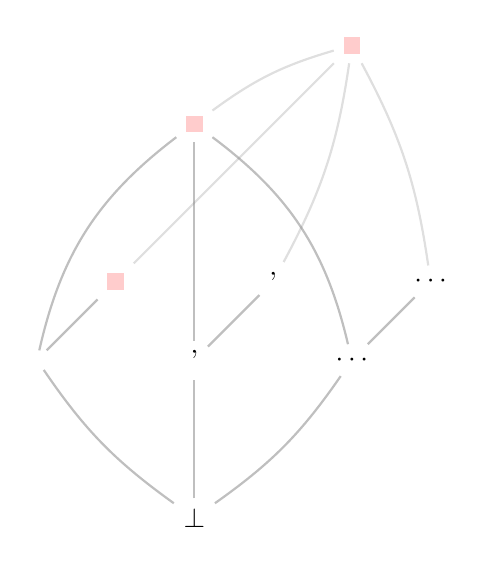
\begin{tikzpicture}
    \node (ub)     at (7,5) {\colorbox{red!20}{\rsub}};
    \node (un)     at (5,4) {\colorbox{red!20}{\unresabbr}};
    \node (rsbs)   at (4,2) {\colorbox{red!20}{\resabbr{\Basesvar}}};
    \node (rsbs')  at (6,2) {\resabbr{\Basesvar'}};
    \node (rsbs'') at (8,2) {$\cdots$};
    \node (orbs)   at (3,1) {\orabbr{\Basesvar}};
    \node (orbs')  at (5,1) {\orabbr{\Basesvar'}};
    \node (orbs'') at (7,1) {$\cdots$};
    \node (bot)    at (5,-1) {$\bot$};

    \path[thick, black, opacity=0.25]
    (bot) edge[bend left=10] node {} (orbs)
    (bot) edge node {} (orbs')
    (bot) edge[bend right=10] node {} (orbs'')
    
    (orbs) edge node {} (rsbs) 
    (orbs') edge node {} (rsbs')
    (orbs'') edge node {} (rsbs'')  
    
    (orbs) edge[bend left=20] node {} (un)
    (orbs') edge node {} (un)
    (orbs'') edge[bend right=20] node {} (un)

    (rsbs) edge[gray] node {} (ub)
    (rsbs') edge[bend right=10, gray] node {} (ub)
    (rsbs'') edge[bend right=10, gray] node {} (ub)

    (un) edge[bend left=10, gray] node {} (ub);
\end{tikzpicture}

\end{frame}


% ----


\begin{frame}[fragile]
\frametitle{Aliasing loads (TMU)}
\begin{itemize}
    \item The fundamental problem with $\unrestricted$ is \textbf{information loss}
    \item Idea: \textbf{remove} $\unrestricted$ entirely and promote $(\onlyread{\Basesvar})$ to $(\onlyread{\textdom{fbas}})$ with $\textdom{fbas} \in \Set{\Bases}$, \ie
    a \textbf{family of sets of bases}
    \begin{itemize}
        \item Every set of the family represents a pointer used for a load \\
        \item if $|\Basesfamvar| > 1$              \qquad the semantics of $\unrestricted$ apply
        \item if $\Basesfamvar = \set{\Basesvar}$ \;   the semantics of $(\onlyread{\Basesvar})$ apply
    \end{itemize}
\end{itemize}
\end{frame}

% ---- 


\begin{frame}[fragile]
\frametitle{Aliasing loads (TMU)}
\begin{minted}[escapeinside=||,mathescape=true]{c}
// Scope $\scope{h}$
void h(int* q, int* restrict r, int* restrict s) {
    *q = *r + |\colorbox{red!20}{*s}|; 
}
\end{minted}
\vspace*{-1cm}
\begin{figure}[!h]
\begin{minipage}[t]{.36\textwidth}

\begin{minted}[escapeinside=||,mathescape=true]{c}
// Scope $\scope{main}$
int main() {
    int x, y;
    int* restrict p = &y;
    *p = 0;
    h(&x, p, p);
}
\end{minted}
\end{minipage}%
\begin{minipage}{.64\textwidth}
\colorbox{red!20}{$\onlyread{\set{\set{(\Blockvar_\text{\textcolor{blue}{$r$}}, \scope{h}), (\Blockvar_p, \scope{main})}}} \joinsym $} \\
\colorbox{red!20}{$\onlyread{\set{\set{(\Blockvar_\text{\textcolor{blue}{$s$}}, \scope{h}), (\Blockvar_p, \scope{main})}}} = ...$}
\\

\executionannotation
{
\{..., \\\  $\Blockvar_r \mapsto \ptr{(\Blockvar_y, \set{(\Blockvar_r, \scope{h}), (\Blockvar_p, \scope{main})})} $, \\
            \ $\Blockvar_s \mapsto \ptr{(\Blockvar_y, \set{(\Blockvar_s, \scope{h}), (\Blockvar_p, \scope{main})})}$ \}
}
{
    \begin{tikzpicture}[stack/.style={rectangle split, rectangle split parts=#1, draw, anchor=center, text centered},
        scope/.style={fill=gray!20, anchor=center}]
    \node[stack=2, minimum width=4.0cm] (s) {
    \nodepart{one} \{$\Blockvar_y \mapsto \onlyread{\set{\set{(\Blockvar_r, \scope{h}), (\Blockvar_p, \scope{main})}}}$\}
    \nodepart{two} \{$\Blockvar_y \mapsto \restricted{\set{(\Blockvar_p, \scope{main})}}$\}
    };
    \node[scope, left=5pt of s.one west]   {\scope{h}};
    \node[scope, left=5pt of s.two west]   {\scope{main}};
    \end{tikzpicture}   
}
\end{minipage}
\end{figure}

\end{frame}


% ---- 


\begin{frame}[fragile]
\frametitle{Aliasing loads (TMU)}
\centering
\colorbox{red!20}{$\onlyread{\set{\set{(\Blockvar_\text{\textcolor{blue}{$r$}}, \scope{h}), (\Blockvar_p, \scope{main})}}} \joinsym \onlyread{\set{\set{(\Blockvar_\text{\textcolor{blue}{$s$}}, \scope{h}), (\Blockvar_p, \scope{main})}}} = ...$}
\\

\begin{minipage}{.43\textwidth}
\begin{itemize}
    \item The updated symmetric \joinsym \ operation (simplified)
    \item $\Basesvar \neq \Basesvar'$
\end{itemize}
\end{minipage}%
\begin{minipage}{.57\textwidth}
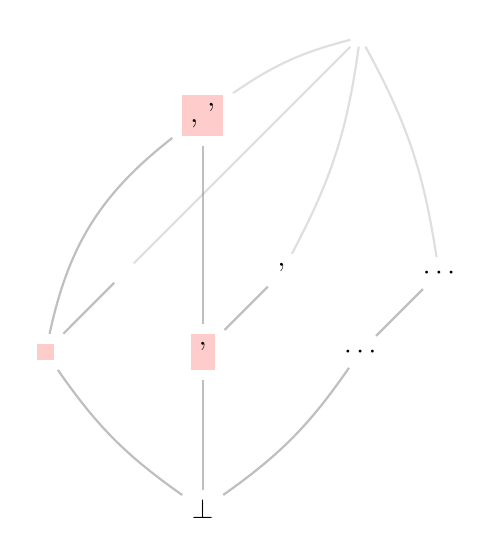
\begin{tikzpicture}
    \node (ub)     at (7,5) {\rsub};
    \node (un)     at (5,4) {\colorbox{red!20}{\orabbr{\set{\Basesvar, \Basesvar'}}}};
    \node (rsbs)   at (4,2) {\resabbr{\Basesvar}};
    \node (rsbs')  at (6,2) {\resabbr{\Basesvar'}};
    \node (rsbs'') at (8,2) {$\cdots$};
    \node (orbs)   at (3,1) {\colorbox{red!20}{\orabbr{\set{\Basesvar}}}};
    \node (orbs')  at (5,1) {\colorbox{red!20}{\orabbr{\set{\Basesvar'}}}};
    \node (orbs'') at (7,1) {$\cdots$};
    \node (bot)    at (5,-1) {$\bot$};

    \path[thick, black, opacity=0.25]
    (bot) edge[bend left=10] node {} (orbs)
    (bot) edge node {} (orbs')
    (bot) edge[bend right=10] node {} (orbs'')
    
    (orbs) edge node {} (rsbs) 
    (orbs') edge node {} (rsbs')
    (orbs'') edge node {} (rsbs'')  
    
    (orbs) edge[bend left=20] node {} (un)
    (orbs') edge node {} (un)
    % (orbs'') edge[bend right=20] node {} (un)

    (rsbs) edge[gray] node {} (ub)
    (rsbs') edge[bend right=10, gray] node {} (ub)
    (rsbs'') edge[bend right=10, gray] node {} (ub)

    (un) edge[bend left=10, gray] node {} (ub);
\end{tikzpicture}
\end{minipage}

\end{frame}




% ---- 


\begin{frame}[fragile]
\frametitle{Aliasing loads (TMU)}
\begin{minted}[escapeinside=||,mathescape=true]{c}
// Scope $\scope{h}$
void h(int* q, int* restrict r, int* restrict s) {
    *q = *r + |\colorbox{red!20}{*s}|; 
}
\end{minted}
\vspace*{-1cm}
\begin{figure}[!h]
\begin{minipage}[t]{.36\textwidth}

\begin{minted}[escapeinside=||,mathescape=true]{c}
// Scope $\scope{main}$
int main() {
    int x, y;
    int* restrict p = &y;
    *p = 0;
    h(&x, p, p);
}
\end{minted}
\end{minipage}%
\begin{minipage}{.64\textwidth}

\executionannotation
{
\{..., \\\  $\Blockvar_r \mapsto \ptr{(\Blockvar_y, \set{(\Blockvar_r, \scope{h}), (\Blockvar_p, \scope{main})})} $, \\
            \ $\Blockvar_s \mapsto \ptr{(\Blockvar_y, \set{(\Blockvar_s, \scope{h}), (\Blockvar_p, \scope{main})})}$ \}
}
{
    \begin{tikzpicture}[stack/.style={rectangle split, rectangle split parts=#1, draw, anchor=center, text centered,align=left},
        scope/.style={fill=gray!20, anchor=center}]
    \node[stack=2, minimum width=4.0cm] (s) {
    \nodepart[align=left]{one} \{$\Blockvar_y \mapsto$ \colorbox{red!20}{$\mathsf{OnlyRead}$ \{} \\
                                \quad \colorbox{red!20}{$\set{(\Blockvar_\text{\textcolor{blue}{$r$}}, \scope{h}), (\Blockvar_p, \scope{main})}$}, \\
                                \quad \colorbox{red!20}{$\set{(\Blockvar_\text{\textcolor{blue}{$s$}}, \scope{h}), (\Blockvar_p, \scope{main})}$ \}} \\ \}
                    
                   
    \nodepart{two} \{$\Blockvar_y \mapsto \restricted{\set{(\Blockvar_p, \scope{main})}}$\}
    };
    \node[scope, left=5pt of s.one west]   {\scope{h}};
    \node[scope, left=5pt of s.two west]   {\scope{main}};
    \end{tikzpicture}   
}
\end{minipage}
\end{figure}

\end{frame}


% ---- 


\begin{frame}[fragile]
\frametitle{Aliasing loads (TMU)}
\begin{minted}[escapeinside=||,mathescape=true]{c}
// Scope $\scope{h}$
void h(int* q, int* restrict r, int* restrict s) {
    *q = *r + *s; 
|\colorbox{red!20}{\}}|
\end{minted}
\vspace*{-1cm}
\begin{figure}[!h]
\begin{minipage}[t]{.36\textwidth}

\begin{minted}[escapeinside=||,mathescape=true]{c}
// Scope $\scope{main}$
int main() {
    int x, y;
    int* restrict p = &y;
    *p = 0;
    h(&x, p, p);
}
\end{minted}
\end{minipage}%
\begin{minipage}{.64\textwidth}

\executionannotation
{
\{..., \\\  $\Blockvar_r \mapsto \ptr{(\Blockvar_y, \set{(\Blockvar_r, \scope{h}), (\Blockvar_p, \scope{main})})} $, \\
            \ $\Blockvar_s \mapsto \ptr{(\Blockvar_y, \set{(\Blockvar_s, \scope{h}), (\Blockvar_p, \scope{main})})}$ \}
}
{
    \begin{tikzpicture}[stack/.style={rectangle split, rectangle split parts=#1, draw, anchor=center, text centered,align=left},
        scope/.style={fill=gray!20, anchor=center}]
    \node[stack=2, minimum width=4.0cm] (s) {
    \nodepart[align=left]{one} \{...,  $\Blockvar_y \mapsto$ $\mathsf{OnlyRead}$ \{ \\
                                \quad $\set{(\Blockvar_\text{\textcolor{blue}{$r$}}, \scope{h}), (\Blockvar_p, \scope{main})}$, \\
                                \quad $\set{(\Blockvar_\text{\textcolor{blue}{$s$}}, \scope{h}), (\Blockvar_p, \scope{main})}$ \} \\ \}
                    
                    
    \nodepart{two} \{$\Blockvar_y \mapsto \restricted{\set{(\Blockvar_p, \scope{main})}}$\}
    };
    \node[scope, left=5pt of s.one west]   {\scope{h}};
    \node[scope, left=5pt of s.two west]   {\scope{main}};
    \end{tikzpicture}   
}
\end{minipage}
\end{figure}

\end{frame}



% ---- 


\begin{frame}[fragile,label=current]
\frametitle{Aliasing loads (TMU)}
\centering

\begin{itemize}
    \item Recall that the restrict rules only apply during the \textbf{scope a restrict pointer is alive}
    \item Filtering: when joining between scopes, remove bases from the expired scope \scope{h}
\end{itemize}

\pause

\begin{tikzpicture}[stack/.style={rectangle split, rectangle split parts=#1, draw, anchor=center, text centered,align=left},
    scope/.style={fill=gray!20, anchor=center}]
\node[stack=2, minimum width=4.0cm] (s) {
\nodepart[align=left]{one} \{$\Blockvar_y \mapsto$ $\mathsf{OnlyRead}$ \{ \\
                            \quad $\set{\text{\colorbox{red!20}{$(\Blockvar_\text{\textcolor{blue}{$r$}}, \scope{h})$}}, (\Blockvar_p, \scope{main})}$, \\
                            \quad $\set{\text{\colorbox{red!20}{$(\Blockvar_\text{\textcolor{blue}{$s$}}, \scope{h})$}}, (\Blockvar_p, \scope{main})}$ \} \\ \}
                
               
\nodepart{two} \{$\Blockvar_y \mapsto \restricted{\set{(\Blockvar_p, \scope{main})}}$\}
};
\node[scope, left=5pt of s.one west]   {\scope{h}};
\node[scope, left=5pt of s.two west]   {\scope{main}};

\draw[->, dashed, thick] (s.one east) to[bend left=90, looseness=3] node[right] {Filter expired bases + $\joinsym$} (s.two east);


\end{tikzpicture}

\leavevmode \\

\begin{itemize}
    \item Filtered state: $\onlyread{\set{\set{(\Blockvar_p, \scope{main})}}}$
    \item $\onlyread{\set{\set{(\Blockvar_p, \scope{main})}}} \joinsym \restricted{\set{(\Blockvar_p, \scope{main})}} = ...$
\end{itemize}

\end{frame}

% ---- 


\begin{frame}[fragile]
\frametitle{Aliasing loads (TMU)}
\centering
\colorbox{red!20}{$\onlyread{\set{\set{(\Blockvar_p, \scope{main})}}} \joinsym \restricted{\set{(\Blockvar_p, \scope{main})}} = \restricted{\set{(\Blockvar_p, \scope{main})}}$}
\\

\begin{minipage}{.43\textwidth}
\begin{itemize}
    \item The updated symmetric \joinsym \ operation (simplified)
    \item $\Basesvar \neq \Basesvar'$
\end{itemize}
\end{minipage}%
\begin{minipage}{.57\textwidth}
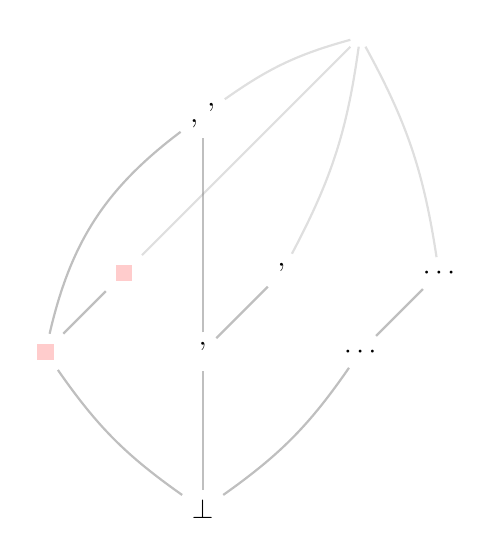
\begin{tikzpicture}
    \node (ub)     at (7,5) {\rsub};
    \node (un)     at (5,4) {\orabbr{\set{\Basesvar, \Basesvar'}}};
    \node (rsbs)   at (4,2) {\colorbox{red!20}{\resabbr{\Basesvar}}};
    \node (rsbs')  at (6,2) {\resabbr{\Basesvar'}};
    \node (rsbs'') at (8,2) {$\cdots$};
    \node (orbs)   at (3,1) {\colorbox{red!20}{\orabbr{\set{\Basesvar}}}};
    \node (orbs')  at (5,1) {\orabbr{\set{\Basesvar'}}};
    \node (orbs'') at (7,1) {$\cdots$};
    \node (bot)    at (5,-1) {$\bot$};

    \path[thick, black, opacity=0.25]
    (bot) edge[bend left=10] node {} (orbs)
    (bot) edge node {} (orbs')
    (bot) edge[bend right=10] node {} (orbs'')
    
    (orbs) edge node {} (rsbs) 
    (orbs') edge node {} (rsbs')
    (orbs'') edge node {} (rsbs'')  
    
    (orbs) edge[bend left=20] node {} (un)
    (orbs') edge node {} (un)
    % (orbs'') edge[bend right=20] node {} (un)

    (rsbs) edge[gray] node {} (ub)
    (rsbs') edge[bend right=10, gray] node {} (ub)
    (rsbs'') edge[bend right=10, gray] node {} (ub)

    (un) edge[bend left=10, gray] node {} (ub);
\end{tikzpicture}
\end{minipage}

\end{frame}


% ---- 


\begin{frame}[fragile]
\frametitle{Aliasing loads (TMU)}
\begin{itemize}
    \item Loads via aliased pointers are now permitted \smiley{}
    \item Achieved our goal of relaxing the semantics for this problem to give \textbf{less UB}, \textbf{consistent} with the ISO standard
\end{itemize}
\end{frame}
